
% !TEX encoding = UTF-8 Unicode
%!TEX root = ../Main/thesis.tex
% !TEX spellcheck = en-US
%%=========================================
\documentclass[../Main/thesis.tex]{subfiles}
\begin{document}
\chapter[Support vector machine coupled with wavelet transform for bearing health monitoring]{Support vector machine coupled with wavelet transform for bearing health monitoring}
\label{sec:waveletandsvm}
Support vector machine for classification are machine learning algorithms that classify vectors into two or more groups, that share some sort of \say{similarity}.
\justify
In this chapter, a purely data driven method is presented. It consists of applying wavelet transform for feature generation, a robust statistical estimator to quantify a bearing health, and a support vector machine (SVM) for anomaly detection. Before giving a detail account of the method, let clarify some semantics and outline the benefits of this method. A feature in the context of this chapter, is a component of a signal. As pointed out earlier, a signal can have multiple components, which can be extracted for example by applying Fourier series or Fourier transform. In this case a feature or component of the original signal is a trigonometric function. A support vector machine (SVM) is a linear classification algorithm for pattern identification that uses margins to separate data into different groups [vapnik1995].
\justify
The method presented in this chapter solely relies on the data to detect any fault. it does not require bearing physical properties, and can be applies to any nonlinear and non-stationary data generated process. In the rest of this chapter we will refer to a generic bearing fault as an anomaly. As defined in [chandola2009], \say{Anomalies are patterns in data that do not conform to a well defined notion of normal behavior}. In section \ref{sec:svm} a detailed account of support vector machine algorithm is lade out, followed by wavelet transform in section \ref{sec:wavelet}. Finally, section \ref{sec:sectionresult} presents a one class SVM coupled with wavelet transform for bearing anomaly detection.

%%%%%%%%%%%%%%%%%%%%%%%%%%%%%%%%%%%%%%%%%%%%%%%%%%%%%%%%%%%%%%%%%%%%%%%%%%%%%%%%%%%%%%%%%%%%%%%%%%%
%%%%%%%%%%%%%%%%%%%%%%%%%%%%%%%%%%%%%%%%%%%%%%%%%%%%%%%%%%%%%%%%%%%%%%%%%%%%%%%%%%%%%%%%%%%%%%%%%%%
\section{Support vector algorithms }
\label{sec:svm}
Support vector algorithms for classification, solve the problem of classifying an input vector into two groups (binary classification), or estimating the distribution of input vector(s). In the context of bearing fault detection: healthy versus unhealthy bearing would be the two groups. The  binary classification is based on optimizing a margin separating the two groups. 
\begin{figure}[H] %  figure placement: here, top, bottom, or page
   \centering
   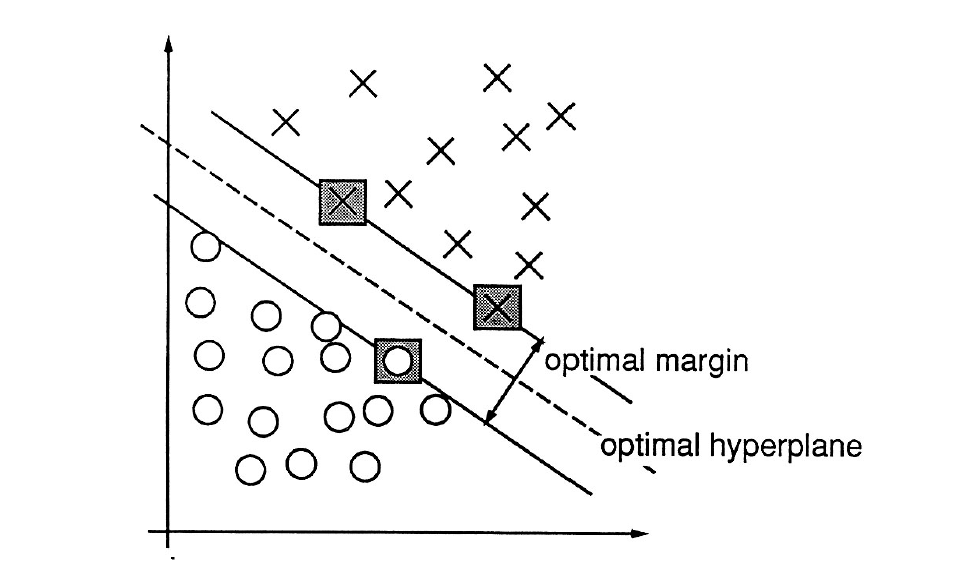
\includegraphics[width=5in]{../fig/svm2d.png} 
   \caption{Illustration of two classes classification from (\cite{vapnik1995})}
   \label{fig:svm2d}
\end{figure}
\justify
Figure \ref{fig:svm2d} shows a two groups classification problem. Two set of points marked by circle and cross are separated by the optimum curve or hyperplane (here the solid dash line). The margin is the distance or gap between solid dark lines. Here the two classes are linearly separable, meaning that a linear function can be used to separate the two classes. Support vectors are points that lies on the margins (points in gray square lying on the dark lines) and defines the margin of largest separation between the two classes.
\justify
The most commonly used and implemented support vector classification algorithms are  C-support vector classification (SVC) (\cite{bosser1992}, \cite{vapnik1995}), $\nu$-support vector classification (\cite{kp2000}) and one-class support vector machine (\cite{kp2001}), for distribution estimation. Here the C-SVC introduces the regularization parameter $C\in (0,\infty)$, while the regularization parameter for the $\nu$-SVC is bounded. Intuitively, the regularization parameter has the effect of decreasing the error for the classification problem.
\justify
The support vector algorithms are formulated as optimization problems in terms of a primal and dual formulation, where each form offers an advantage in the derivation of the solution, and on the computer implementation level. In addition, the relationship between the dual formulation and the primal formulation allows a derivation of the solution of the optimization problem. 


\subsection{C-Support vector classification (SVC)}
Let $\bm{x} = \{ \bm{x}_{i}\}$ be training examples, $\bm{x}_{i}\in \mathbb{R}^{n}, i = 1, \cdots, m$ and $y_{i}\in \{1,-1\}$ be the classes , $\bm{y} = \{ y_{i} \}$. The C-SVM (\cite{bosser1992}, \cite{vapnik1995}) solves the primal optimization problem
\begin{equation}
	\min_{w,b,\xi} \quad \frac{1}{2}\bm{w}^{T}\bm{w} + C\sum_{i = 1}^{m}\xi_{i}
\end{equation}
subjected to 
\begin{equation}
	y_{i}(\bm{w}^{T}\phi(\bm{x}_{i}) + b) \geq 1 - \xi_{i}
\end{equation}
\begin{equation}
	\xi_{i} \geq 0, \quad i = 1, \cdots, m
\end{equation}
where $\phi(x_{i})$ maps $x_{i}$ in higher dimension space and the constant $C > 0$ is a real number which is called regularization parameter.
Because of \say{the possible high dimensionality of the vector $\bm{w}$, the following dual problem} is solved (\cite{chang2001}):
\begin{equation}\label{eq:cdual1}
	\min_{\alpha}\quad g(\bm{\alpha}) = \frac{1}{2}\bm{\alpha}^{T}Q\bm{\alpha}-\bm{e}^{T}\bm{\alpha}, \quad \bm{\alpha}=\{\alpha_{i}\}, i=1,\cdots,m
\end{equation}
subjected to 
\begin{equation}\label{eq:cdual2}
	\bm{y}\bm{\alpha}^{T} = 0. \quad 0 \leq \alpha_{i} \leq C,\quad  i = 1,\cdots, m
\end{equation}
\justify
where $g(\bm{\alpha})$ is called the dual function, $\bm{y}\in \mathbb{R}^{m}$ is the indicator vector, $\bm{e} = [1,\cdots,1]^{T}$, $Q$ is the semi-definite matrix
\begin{equation}\label{eq:Q}
	Q_{ij} = y_{i}y_{j}K(\bm{x}_{i},\bm{x_{j}})
\end{equation}
and $K$ is the kernel function 
\begin{equation}
	K(\bm{x}_{i},\bm{x}_{j}) = \phi(\bm{x}_{i})^{T}\phi(\bm{x}_{j})
\end{equation}
\begin{equation}
K: \mathbb{R}^{d}\times \mathbb{R}^{d} \rightarrow \mathbb{R}
\end{equation}
that  maps the data into a higher dimension space. Example of common Kernel functions are 
\begin{itemize}
	\item Linear kernel,  $K\left(x,z\right) = x^{T}z$
	\item Polynomial of degree $q$ kernel, $K\left(x,z\right) = \left(1+x^{T}z\right)^{q}$ 
	\item Exponential kernel,  $K(x,z) = \exp\left(-\gamma ||x-z||\right)$ ,$\gamma\in\mathbb{R}$
	\item Gaussian kernel,  $K(x,z) = \exp\left(-\gamma ||x-z||^{2}\right)$ ,$\gamma\in\mathbb{R}$
\end{itemize}

\begin{figure}[H] %  figure placement: here, top, bottom, or page
   \centering
   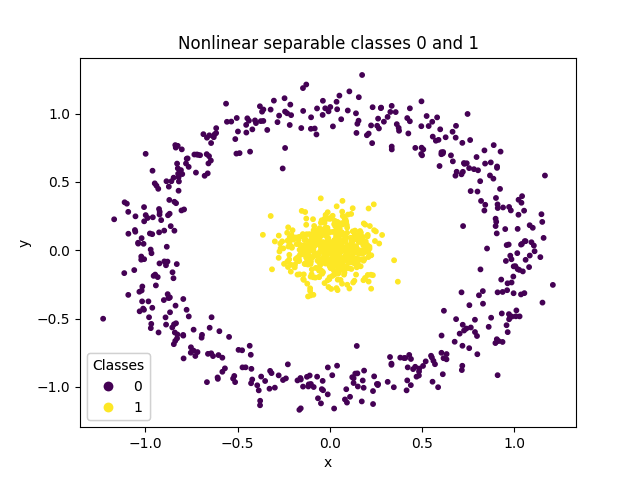
\includegraphics[width=4in]{../fig/nonlinearseparable.png} 
   %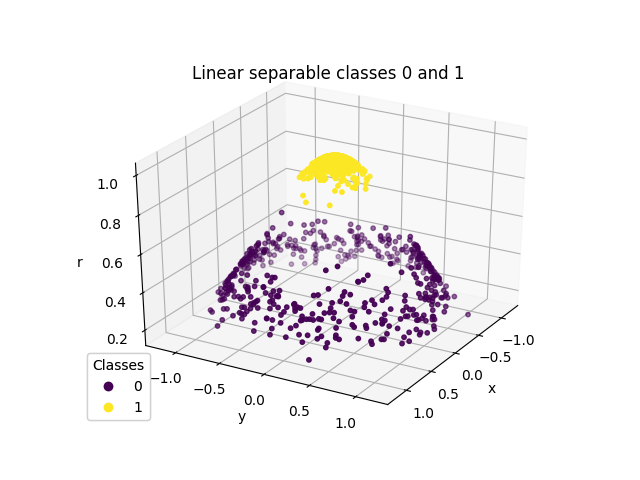
\includegraphics[width=4in]{../fig/linearseparable.png} 
   \caption{Nonlinear separable classes 0 and 1}.
   \label{fig:kernelsvm}
\end{figure}

\begin{figure}[H] %  figure placement: here, top, bottom, or page
   \centering
   %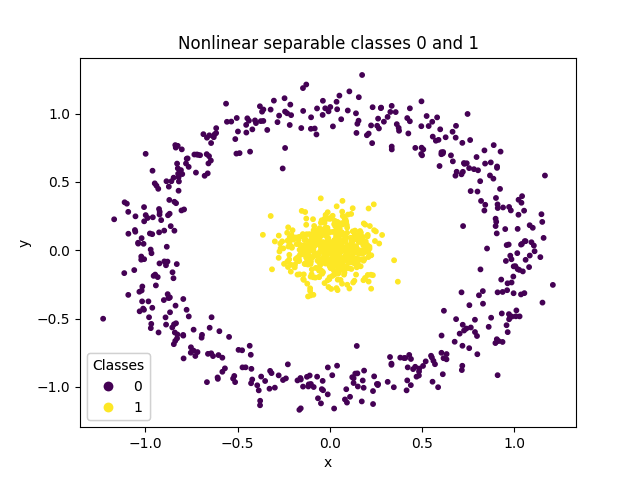
\includegraphics[width=4in]{../fig/nonlinearseparable.png} 
   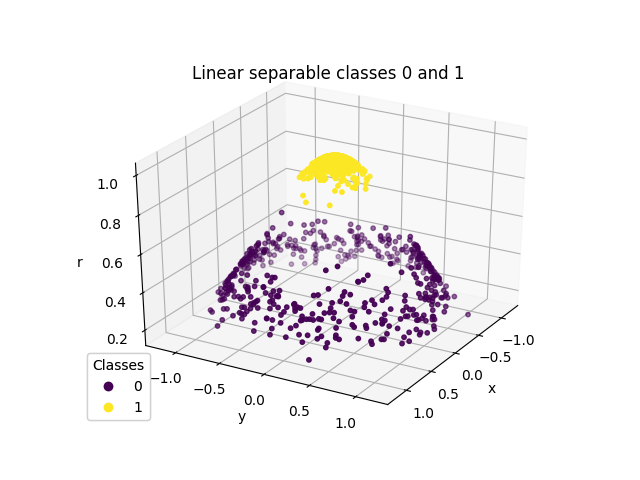
\includegraphics[width=4in]{../fig/linearseparable.png} 
   \caption{Linear separable classes 0 and 1 after using a Gaussian kernel to map the data in higher dimension}.
   \label{fig:kernelsvm1}
\end{figure}
\justify
The effect of a kernel function can be seen in Figure \ref{fig:kernelsvm} and \ref{fig:kernelsvm1}. In Figure \ref{fig:kernelsvm}, the data has two classes that can not be linearly separated directly. To linearly separate the classes, a Gaussian kernel is used to project the data in a higher dimension, which can be seen in Figure \ref{fig:kernelsvm1}.
\justify
The relationship between the primal and the dual problem is that, the dual function is a lower bound of the optimal solution $\bm{w}$ (\cite{boyd2004}), that is 
\begin{equation}
	g(\bm{\alpha}) \leq \bm{w},
\end{equation}
but since the primal optimization problem is convex, we have equality (\cite{boyd2004}), that is 
\begin{equation}\label{eq:rdual}
g(\bm{\alpha}) = \bm{w}.
\end{equation}
The solution of the dual problem (\ref{eq:cdual1}, \ref{eq:cdual2}) coupled with the primal-dual relationship (\ref{eq:rdual}) gives the optimal $\bm{w}$ (\cite{chang2001}) as
\begin{equation}
	\bm{w} = \sum_{i = 1}^{m}y_{i}\alpha_{i}\phi(\bm{x}_{i})
\end{equation}
where the decision boundary is given by
\begin{equation}
	sgn\left(\bm{w}^{T}\phi(\bm{x}) + b  \right) = sgn\left(  \sum_{i=1}^{m}y_{i}\alpha_{i}K(\bm{x}_{i},\bm{x} ) +b    \right)
\end{equation}
where sgn is the sign function. The decision boundary is used to separate classes.

\subsection{$\nu$-Support vector classification (SVC)}
The $\nu$-SVC (\cite{kp2000}), formulates the binary classification problem in term of a bounded regularization
 parameter $\nu$, as opposed to the C-SVC where the regularization parameter C, can take any positive real number $C\in (0,\infty)$. The parameter $\nu$ is \say{an upper bound on the fraction of training errors and a lower bound of the fraction of support vectors} (\cite{chang2001}). 
 \justify
 For the $\nu$-SVC the primal optimization problem is (\cite{chang2001})
 \begin{equation}
 \min_{w,b,\xi,\rho} +\quad \frac{1}{2}\bm{w}^{T}\bm{w}- \nu\rho + \frac{1}{m}\sum_{i = 1}^{m}\xi_{i}
 \end{equation}
 subjected to 
 \begin{equation}
 y_{i}(\bm{w}^{T}\phi(\bm{x}_{i}) + b) \geq \rho - \xi_{i}, \quad \xi_{i} \geq 0, \quad i = 1,\cdots,m \quad, \rho \geq 0
 \end{equation}
 and the corresponding dual is 
 \begin{equation}\label{eq:nudual1}
 \min_{\alpha}\quad \frac{1}{2}\bm{\alpha}^{T}Q\bm{\alpha}
 \end{equation}
 subjected to 
 \begin{equation}\label{eq:nudual2}
  0 \leq \alpha_{i} \leq \frac{1}{m},\quad  i = 1,\cdots, m, \quad \bm{e}^{T}\bm{\alpha} \geq \nu, \quad \bm{y}^{T}+\bm{\alpha} = 0
 \end{equation}
 where $Q$ is defined in equation (\ref{eq:Q}) and the decision boundary is given by
 \begin{equation}
 	sgn\left(  \sum_{i=1}^{m}y_{i}\alpha_{i}K(\bm{x_{i}},\bm{x}) +b\right)
 \end{equation}
 
 \subsection{One-class support vector machine (SVM)}
 The C-support vector classification and the $\nu$.support vector classification on deal with binary classification or two class classification problems. However, they might be situations where one is only concerned in estimating the distribution of data. The One-class support vector machine (\cite{kp2001}) was designed to address this issue.
 it solves the dual  (\cite{chang2001})
 
 \begin{equation}
 \min_{w,b,\xi,\rho} +\quad \frac{1}{2}\bm{w}^{T}\bm{w}- \rho + \frac{1}{\nu m}\sum_{i = 1}^{m}\xi_{i}
 \end{equation}
 subjected to 
 \begin{equation}
 \bm{w}^{T}\phi(\bm{x}_{i}) \geq \rho - \xi_{i}, \quad \xi_{i} \geq 0, \quad i = 1,\cdots,m \quad
 \end{equation}
 and the corresponding dual is 
 \begin{equation}\label{eq:onedual1}
 \min_{\alpha}\quad \frac{1}{2}\bm{\alpha}^{T}Q\bm{\alpha}
 \end{equation}
 subjected to 
 \begin{equation}\label{eq:onedual2}
 0 \leq \alpha_{i} \leq \frac{1}{m\rho},\quad  i = 1,\cdots, m, \quad \bm{e}^{T}\bm{\alpha} = 1
 \end{equation}
 where $Q$ is defined in equation (\ref{eq:Q}) and the decision boundary is given by
 \begin{equation}
 sgn\left(  \sum_{i=1}^{m}\alpha_{i}K(\bm{x_{i}},\bm{x}) -\rho \right)
 \end{equation}
 
%%%%%%%%%%%%%%%%%%%%%%%%%%%%%%%%%%%%%%%%%%%%%%%%%%%%%%%%%%%%%%%%%%%%%%%%%%%%%%%%%%%%%%%%%%%%%%%%%%%
%%%%%%%%%%%%%%%%%%%%%%%%%%%%%%%%%%%%%%%%%%%%%%%%%%%%%%%%%%%%%%%%%%%%%%%%%%%%%%%%%%%%%%%%%%%%%%%%%%%
\section{An overview of wavelet transform}
\label{sec:wavelet}
The appearance of a crack in a bearing, generates short duration periodic high frequency pulses. The Fourier transform is not well equip to detect the time of occurrence of the pulses, since it only provides frequency and amplitude information. A better approach could be the short-time Fourier transform, where the entire interval is divided into small subintervals. The Fourier transform can then be applied on each subinterval. However, this method does not accurately detect the time at which the pulses occur, since the Fourier basis function are not localized in time, \cite{albert09}. And there comes the wavelet transform in the scene.  
\begin{figure}[H] %  figure placement: here, top, bottom, or page
   \centering
   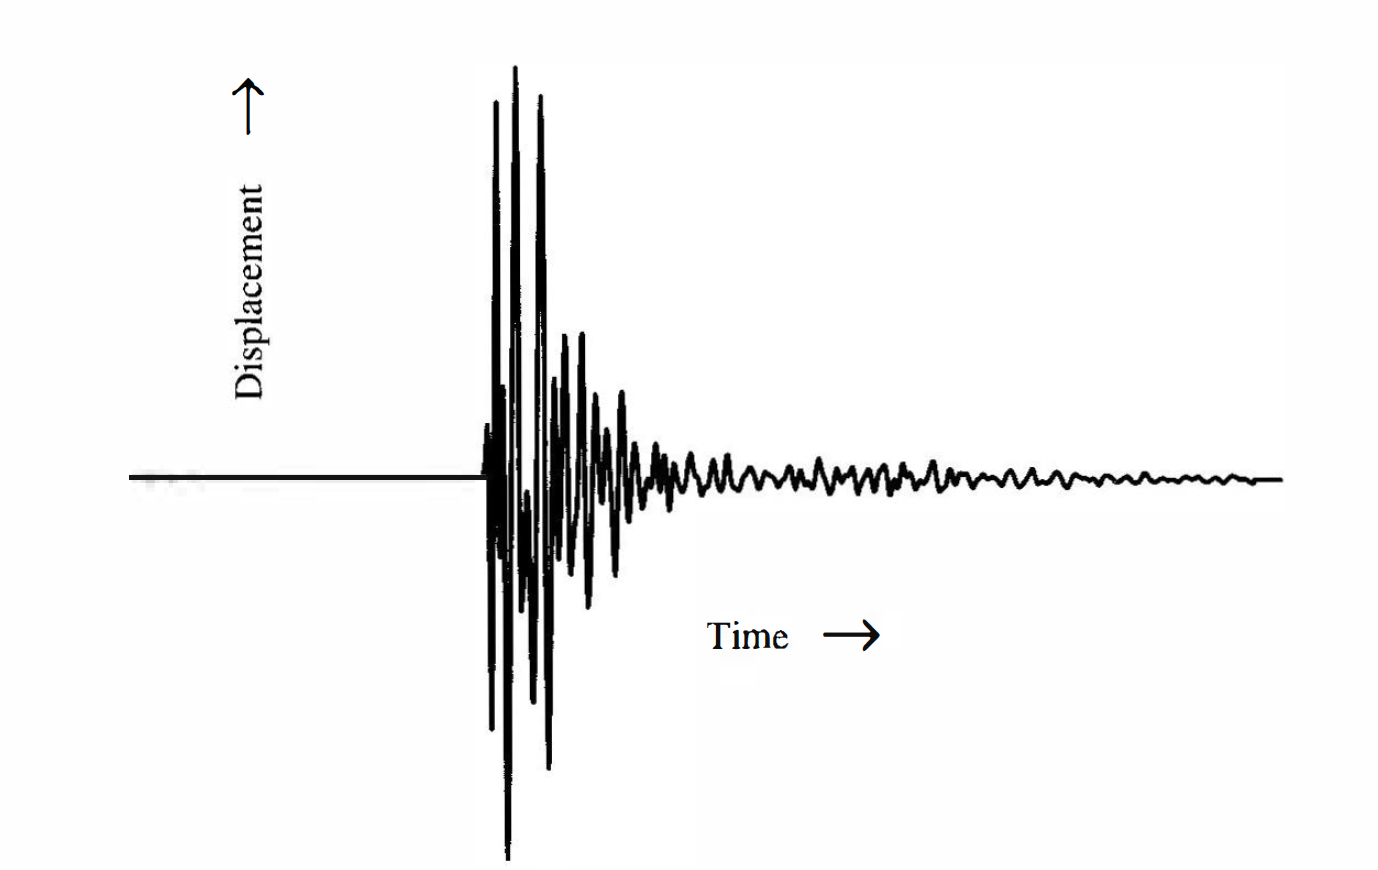
\includegraphics[width=4.5in]{../fig/seismicwave.png} 
   \caption{Example of a seismic trace. Taken from \cite{albert09}}
   \label{fig:seismicwave}
\end{figure}
\justify
Wavelet transform is a signal analysis tool that decomposes a signal into its subcomponents by using orthonormal and (sometime localized) basis functions called wavelets. The latter were originally applied in seismic survey in order to detect seismic trace \cite{albert09}. Figure \ref{fig:seismicwave} shows a seismic trace, which is a decaying high frequency short duration pulse, generated by a ground movement. Wavelets can detect and encode temporal and frequency information, unlike the Fourier transform. By construction, wavelets can \say{zoom in to observe} high frequency event and \say{zoom out} to record long and slow oscillatory movement. They can approximate non-stationary and nonlinear signal efficiently. This ability to adapt to time and space variation is due to a scaling factor build in the heart of wavelets.
\justify
Technically speaking, wavelets are family of functions generated by two functions: a scaling function denoted by $\phi$ and a wavelet function $\psi$. The former and latter are sometime refer to as \say{father wavelet} and \say{mother wavelet} respectively. By combining the scaling function and the wavelet function, one can approximate, as well as decompose a target function (signal) into its various frequency components, and analyze them with respect to different scale or resolution. In this thesis we are interested in families of wavelets with compact support, also refer to as localized. By definition, the support of a function is a subset of the function domain, where the function does not equal to zero, but equal zero everywhere else. Being localized, these wavelets can model local short time high frequency event such as pulses emitted by a crack in a bearing. The most celebrated localized wavelet family are the Debauchies wavelets. 
\justify
The simplest wavelet belonging to the Debauchies wavelets family is the Haar wavelet, also known as Db1. The latter is the only discontinuous wavelet in that hierarchy of wavelets.
The Haar scaling function $\phi$ and the Haar wavelet function $\psi$ are given by
\begin{equation}\label{eq:haar-wavelet}
\begin{split}
\phi(x) &=
  \begin{cases}
   1 & \text{ if $0 \leq t \le 0$} \\
    0 & \text{otherwise}\\
  \end{cases}\\
\psi(t)& =
  \begin{cases}
   1 & \text{ if $0 \leq t \le \frac{1}{2}$ } \\
    -1 & \text{ if  $\frac{1}{2} \leq t \le 1$ }\\
    0 & \text{otherwise},
  \end{cases}
  \end{split}
\end{equation}
and Figure \ref{fig:haar-phi} and \ref{fig:haar-psi} show their graphical representation with discontinuities specified by blue bold points. The Haar wavelet function can also be written in  terms of the scaling function as 
\begin{equation}
\psi(t) = \phi(2x)-\phi(2x-1) \nonumber.
\end{equation}
\begin{figure}[H] %  figure placement: here, top, bottom, or page
   \centering
   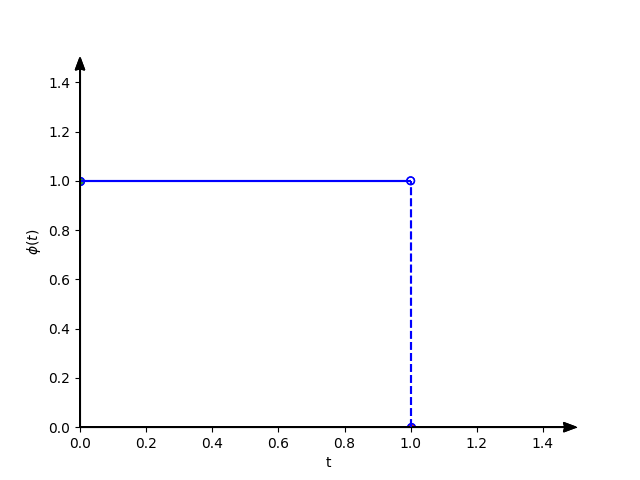
\includegraphics[width=4in]{../fig/haar-phi.png} 
   \caption{Graphical representation of Haar scaling function $\phi$ along the time scale $t$}
   \label{fig:haar-phi}
\end{figure}
\begin{figure}[H] %  figure placement: here, top, bottom, or page
   \centering
   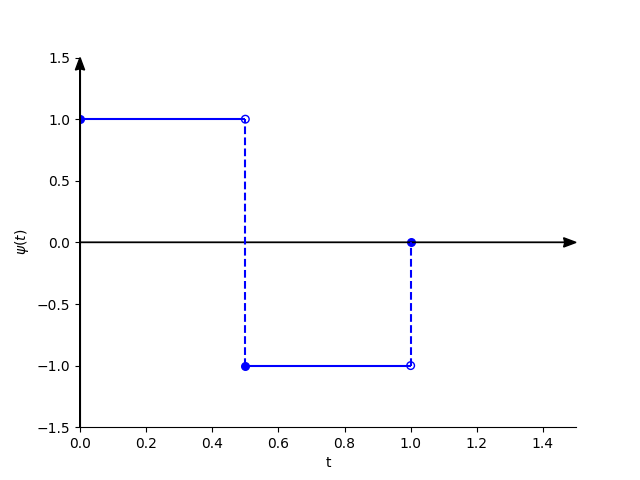
\includegraphics[width=4in]{../fig/haar-psi.png} 
   \caption{Graphical representation of Haar wavelet function $\psi$ along the time scale $t$}
   \label{fig:haar-psi}
\end{figure}
\clearpage
\justify
In wavelet transform, multi-resolution analysis is concerned with decomposing a signal into it frequency components, and look at the different components with respect to a target time scale or resolution. As such, wavelet transform is a function approximation apparatus, which keeps track of frequency and temporal information. In this framework, we can conceptualize the scaling function $\phi$ as encoding temporal information, whereas the wavelet function $\psi$ encapsulates frequency information. In the mathematical framework of function approximation, one needs a vector space and a basis function in order to express a target function in terms on the basis function in the chosen vector space.
\justify
In terms of the Haar scaling function and the wavelet function, we can construct two orthonormal basis given by 
\begin{equation}\label{eq:basis-phi}
\left\{\phi_{j,k} = 2^{\left(\frac{j}{2}\right)}\phi\left( 2^{j}t-k \right), k\in\mathbb{Z}, \quad j = 0,1 \cdots,n  \right\}
\end{equation}
\justify
\begin{equation}\label{eq:basis.psi}
\left\{\psi_{j,k} = 2^{\left(\frac{j}{2}\right)}\psi\left( 2^{j}t-k \right), k\in\mathbb{Z}, \quad j = 0,1 \cdots,n \right\},
\end{equation}
and construct the vector spaces
\begin{equation}
\mathcal{V}_{j} = \text{Spann}\left\{ \phi_{j,k}  \right\}
\end{equation}
\begin{equation}
\mathcal{W}_{j} = \text{Spann}\left\{ \psi_{j,k}  \right\}.
\end{equation}
The Haar decomposition theorem allows one to approximate a target function $g$ as
\begin{equation}
g_{j}(t) = \sum_{k\in\mathbb{Z}}a_{k}^{j}\phi\left(  2^{j}t-k\right)\in \mathcal{V}_{j}
\end{equation} 

\begin{equation}
w_{j-1}(t) = \sum_{k\in\mathbb{Z}}d_{k}^{j}\psi\left(2^{j-1}t-k\right)\in\mathcal{W}_{j-1}
\end{equation}
\begin{equation}
g_{j-1}(t) = \sum_{k\in\mathbb{Z}}a_{k}^{j}\phi\left(2^{j-1}t-k\right)\in\mathcal{V}_{j-1}
\end{equation}
where the wavelets coefficients $a_{k}^{j-1}$ and $d_{k}^{j-1}$ are related as also called approximate and detail coefficient 
\begin{equation}
d_{k}^{j-1} = \frac{a_{2k}^{j}-a_{2k+1}^{j}}{2}, \quad a_{k}^{j-1} = \frac{a_{2k}^{j}+a_{2k+1}^{j}}{2}
\end{equation}
Now the target function can be decomposed in terms of its frequency components as 
\begin{equation}
g_{j}(t) = w_{j-1}(t) +  w_{j-1}(t)+\cdots + g_{0}(t)
\end{equation}
In approximating a signal over an interval, $2^{j}$ is the number of discretized points and the mesh size is $\frac{1}{2^{j}}$. 
for discrete signal this we have the discrete wavelet transform given by :
\begin{equation}
g = a + d
\end{equation}
the fast wavelet transform allows fast computation...
In the next section we apply the Debauchies wavelet combined with the support vector machine defined in section \ref{sec:svm} to detect bearing faults
%%%%%%%%%%%%%%%%%%%%%%%%%%%%%%%%%%%%%%%%%%%%%%%%%%%%%%%%%%%%%%%%%%%%%%%%%%%%%%%%%%%%%%%%%%%%%%%%%%%
%%%%%%%%%%%%%%%%%%%%%%%%%%%%%%%%%%%%%%%%%%%%%%%%%%%%%%%%%%%%%%%%%%%%%%%%%%%%%%%%%%%%%%%%%%%%%%%%%%%
\clearpage
\section{Coupled SVM and wavelet transform for bearing anomalies detection: A case study}
\label{sec:result-svm-wavelet}
In section \ref{sec:svm} and \ref{sec:wavelet}, we described support vector machine as a linear classifier, and wavelet transform as a signal decomposition tool. In this section, we present a methodology that couples SVM and wavelet transform. The objective is to monitor and detect bearing failure, for a system of bearings mounted on a motor. The data used in this case study was generated in the experimental set up described in Chapter 2. In this experiment, a motor rotating at 2000 rotations per minute and housing four bearings, was run to failure. At the end of the experiment, bearing number one was severely affected by a defect in the outer ring.
\justify
The present methodology, for bearing fault monitoring and detection, consists of three successive steps. In the first step, an input signal is decomposed into two sub-signals by applying a wavelet transform. The two sub-signals are the approximate coefficients and the detailed coefficients. The former and the latter can be interpreted in two ways. Firstly, they represent the low and high frequency information for a signal, and secondly they encode the temporal and frequency information. We will refer to them as temporal and frequency features, respectively. 
\justify
In the second step of the methodology, the inter quartile range of the temporal and frequency features are computed. The inter quartile range represents the health index of a bearing. Recall that the inter quartile range is a statistical estimator, that quantifies the dispersion of a sample. It is a robust estimator in the sense that is is based on the median. The asymptotic breaking point of the median is one-half $\left(\frac{1}{2}\right)$, as opposed to the mean whose asymptotic breaking point is zero. \say{The asymptotic breaking point represents the fraction of data point that can be given arbitrary values without making an estimator arbitrary bad}. In the case of the mean for example, even one \say{bad} data point such as an outlier can distort an estimator based on the mean. On the other hand, since the inter quartile range is based on the median, even if half of the data is \say{bad}, we can still rely on the values of an estimator based on the median. 
\justify
In the third and last step, we apply the support vector machine classifier. For successive bearings measurement sample, we apply step one and step two to generate a set of points in the temporal and frequency feature space. Each point represents the health index coordinate, and together the points represent the health trajectory of a bearing. Once we have the health index trajectory we apply the SVM.
\begin{figure}[H] %  figure placement: here, top, bottom, or page
   \centering
   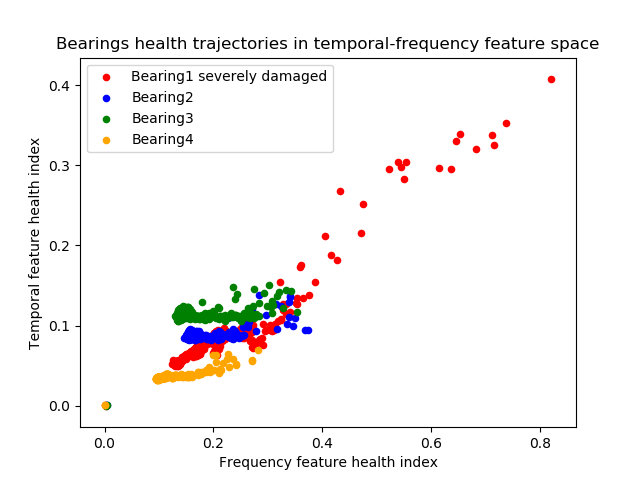
\includegraphics[width=5in]{../fig/health_plot.png} 
   \caption{Health trajectories of all bearing mounted on a motor run to failure at 2000 rotation per minute}
   \label{fig:health_plot}
\end{figure}

\begin{figure}[H] %  figure placement: here, top, bottom, or page
   \centering
   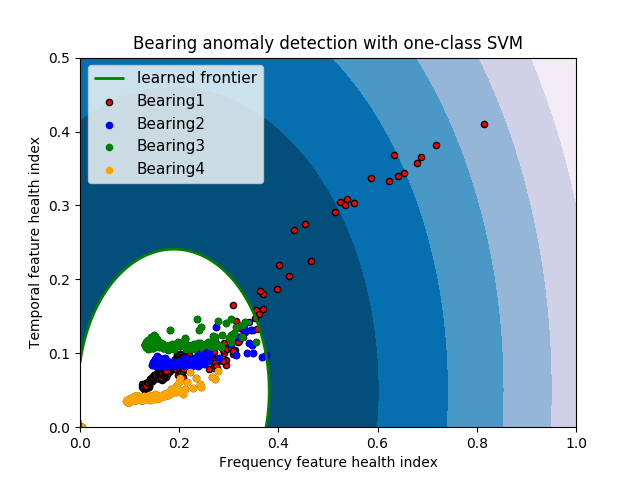
\includegraphics[width=5.3in]{../fig/svm.png} 
   \caption{One class support vector machine }
   \label{fig:one-class-svmt}
\end{figure}
\begin{figure}[H] %  figure placement: here, top, bottom, or page
   \centering
   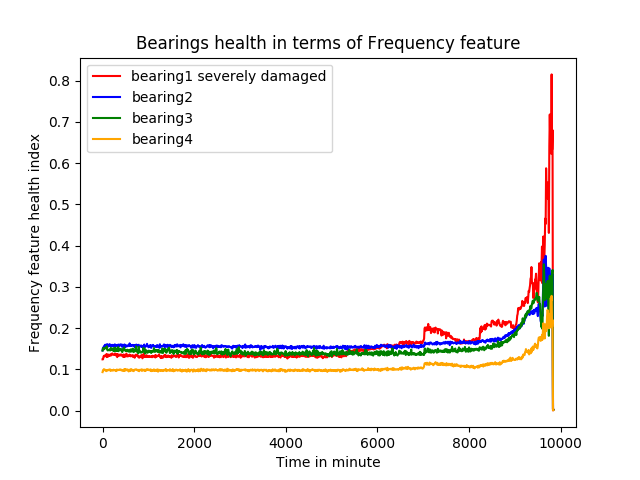
\includegraphics[width=5.3in]{../fig/frequency_feature_health.png} 
   \caption{Frequency feature health index as a function of time-}
   \label{fig:frequency_feature_health}
\end{figure}

\begin{figure}[H] %  figure placement: here, top, bottom, or page
   \centering
   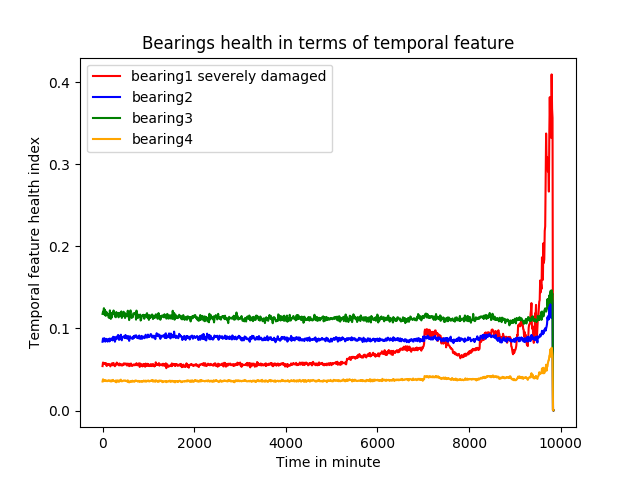
\includegraphics[width=5.3in]{../fig/temporal_feature_health.png} 
   \caption{Temporal feature health index as a function of time-}
   \label{fig:temporal_feature_health}
\end{figure}




















%%%%%%%%%%%%%%%%%%%%%%%%%%%%%%%%%%%%%%%%%%%%%%%%%%%%%%%%%%%%%%%%%%%%%%%%%%%%%%%%%%%%%%%%%%%%%%%%
\blankpage
\end{document}

